\documentclass[12pt]{article}
%\documentclass[10pt,letterpaper]{article}
\usepackage[letterpaper]{geometry}
\usepackage[utf8]{inputenc}
\usepackage[english]{babel}
\usepackage{graphicx}
\usepackage{cancel}
\usepackage{amsmath}
\usepackage{ulem}
\usepackage{authblk}
\usepackage{indentfirst}
\usepackage{enumitem}
\usepackage{cancel}
\usepackage{soul}
\newenvironment{QandA}{\begin{enumerate}[label=\bfseries\arabic*.]\bfseries}
                      {\end{enumerate}}
\newenvironment{answered}{\par\quad\normalfont}{}

\title{CIS501: Branch Prediction}
\author[1]{Shreyas S. Shivakumar}

\begin{document}

\maketitle

\section{Lecture Notes}

\begin{QandA}
\item Control Dependencies
\begin{answered}
    We haven't talked about \textbf{control hazards} yet, i.e when we have some control flow instruction coming through the pipeline that dictates what instruction should follow it. It can be thought of as a dependency through the \textbf{Program Counter (PC)} since the \textbf{PC} dictates the order of instruction flow. 
    
    \qquad\textbf{Branch Prediction} is how we will attempt to solve this problem. Branch Prediction cannot however fix all cases of failure related to control hazards. 
\end{answered}

\item What are the challenges with Branch instructions?
\vspace{-0.85cm}
\begin{answered}
\begin{itemize}
    \item First, when an instruction is coming down the pipeline, we first need to figure out whether it is a \textbf{BR} instruction or not. This doesn't happen during the \textit{Fetch Stage} but happens during the \textit{Decode Stage}.
    
    \item Second, we need to figure out which way the \textbf{BR} instruction should go, i.e should the processor move to the next sequential instruction or should it jump to the \textit{target}. This usually involves some computation to figure out what the \textit{target} address is, and thus involves the \textbf{ALU}. So this starts to illustrate that some of the information that we need is computed later into the pipeline.
    
    This gap between \textit{when I need the information} and \textit{when I have it} is the primary problem here and indicates that there will probably be some \textbf{stalling} involved.
    
    \item Lastly, building upon the first challenge - when the processor is handling a Branch instruction, it is usually Fetched and then moves onto the \textit{Decode Stage}. But what should we be doing in the \textit{Fetch Stage} next? Logically, we will have to fetch the next instruction in the sequence. But if the previous instruction was indeed a \textbf{Branch} instruction, we should be going to the \textit{target} in the next cycle instead of the next sequential instruction. This is another fundamental problem in handling \textbf{Branch} instructions. \textit{We don't yet know what the right thing to do is, but we have to do something!}. We can \textit{not do anything} but that would then indicate a 3 cycle stall/gap, which isn't good for performance.
\end{itemize}
\end{answered}

\item How do we then fix this problem?
\begin{answered}
    We can just \textbf{guess}. In our previous approach of handling \textit{data hazards}, we would try to identify a problem early on and make arrangements to avoid that problem or minimize it's effects on the system. However, with \textit{control hazards}, we take a different approach because \textbf{waiting/stalling} is too expensive. We instead \textbf{guess}, and hope to make a \textbf{smart guess}. This does not guarantee that we are always correct, so when we are wrong we must ensure there are mechanisms in place to clean up behind us. This is the idea behind \textbf{Speculative Execution}.
\end{answered}

\item Speculative Execution
\vspace{-0.85cm}
\begin{answered}
\begin{itemize}
    \item Execute before all parameters are known with certainty
    \item If your speculation is \textit{correct}, you have avoided stalls and improved performance significantly
    \item If your speculation is \textit{incorrect} (mis-speculation), you have to fix what you broke by flushing all incorrect instructions and undo all incorrect changes, going back to the original state
\end{itemize}
\end{answered}

\item Control Speculation
\begin{answered}
    This is the first type of speculation we will introduce. When you have a control flow instruction, you don't know where it is going, so the speculation is made on the control flow path. 
    \begin{itemize}
        \item We want to guess whether it is a \textbf{Branch Instruction} to begin with.
        \item If it is a \textit{Branch Instruction}, we want to guess whether it is \textbf{taken}.
        \item If it is \textit{taken}, we want to guess what it's \textbf{target} is.
    \end{itemize}
    This ultimately results in guessing \textit{where should I go next} or more simply \textit{what is the next \textbf{PC} that I should be going to?}
    
    According to this, what we've been doing so far is also technically \textit{speculation}, except we guessed that the next \textbf{PC} would always be \textbf{PC + 4}.
\end{answered}

\item At what stage should we perform Branch Prediction?
\begin{answered}
    Ideally, the later we do it, the more accurate our prediction will be since we will have more and more information available to us as we go down the pipeline. But this is not necessarily good for performance since it will ensure that some cycles are lost in case the branch was actually taken.
    
    \textbf{1. During Decode:}
    
    \textit{Pros:}
    
    If we do it after the decoding operation, we have a lot more information - we know if it is indeed a \textit{Branch Instruction} or a \textit{Jump Instruction} etc. This will help quite a bit for example if it is a \textit{Jump Instruction}, we know that it is always taken and we can update our PC accordingly. Even if it is a simple \textit{Add Instruction}, it is useful because then we don't need to make any exotic guesses and we can just update the PC to the next sequential address. 
    
    \textit{Cons:}
    
    Even at it's best, this will introduce a one cycle penalty. 
    \begin{center}
    \begin{tabular}{ |c|c|c|c|c|c|c|c|c|c| } 
     \hline
     Cycle & 1 & 2 & 3 & 4 & 5 & 6 & 7 & 8 & 9\\ 
     \hline
     BNEZ R3, target & F & D & X & M & W & - & - & - & -\\ 
     target: ADD R5, R4 $\rightarrow$ R4 & - & ? & F & D & X & M & W & - & - \\ 
     \hline
    \end{tabular}
    \end{center}   
    
    \textbf{2. During Fetch:}
    
    \textit{How would this work?}
    
    Realistically, we don't really know anything about the instruction during the \textit{Fetch Stage}. But we will design mechanisms that will make this possible.
\end{answered}

\item Branch Recovery
\begin{answered}
    How do we handle recovering from when a \textit{Branch Instruction} is actually \textbf{taken}, i.e we figured this out in the \textit{Execute Stage}? The instructions that are in the \textit{Fetch Stage} and the \textit{Decode Stage} are now \textbf{wrong}. These instructions need to be \textit{flushed}; this can be done by replacing them with \textbf{no-ops}. Not too much damage has been done since these instructions haven't written anything to permanent state elements (register files, memory) yet. The \textit{Program Counter} has however changed, but this is easier to fix. This exercise does introduce a \textbf{two cycle penalty} for any \textit{Branch Instruction} that is \textbf{taken}. 
    
    For \textit{example:} in \textbf{Lab 4} where we implement a Pipelined LC4 processor without \textit{Branch Instructions}, we always predict PC = PC + 1, but when this is wrong, we need to perform branch recovery and introduce the respective stall cycles. This is done by just adding a MUX that can switch between a \textit{no-op} signal and the regular instruction. 
    
    \textit{Speculation:}
    
    \begin{center}
    \begin{tabular}{ |c|c|c|c|c|c|c|c|c|c| } 
     \hline
     Cycle & 1 & 2 & 3 & 4 & 5 & 6 & 7 & 8 & 9\\ 
     \hline
     ADDI R1, 1 $\rightarrow$ R3 & F & D & X & M & W & - & - & - & -\\ 
     BNEZ R3, targ & - & F & D & \textbf{\underline{X}} & M & W & - & - & - \\ 
     STORE R6 $\rightarrow$ [R7, 4] & - & - & \textit{F} & \textit{D} & \textit{X} & \textit{M} & \textit{W} & - & - \\ 
     MUL R8, R9 $\rightarrow$ R10 & - & - & - & \textit{F} & \textit{D} & \textit{X} & \textit{M} & \textit{W} & - \\ 
     \hline
    \end{tabular}
    \end{center}       
    
    We realize where we are actually heading in \textit{Cycle 4}!
    
    \textit{Recovery:}
    \begin{center}
    \begin{tabular}{ |c|c|c|c|c|c|c|c|c|c| } 
     \hline
     Cycle & 1 & 2 & 3 & 4 & 5 & 6 & 7 & 8 & 9\\ 
     \hline
     ADDI R1, 1 $\rightarrow$ R3 & F & D & X & M & W & - & - & - & -\\ 
     BNEZ R3, targ & - & F & D & \textbf{\underline{X}} & M & W & - & - & - \\ 
     \st{STORE R6 $\rightarrow$ [R7, 4]}& - & - & \textit{\st{F}} & \textit{\st{D}} & -- & -- & -- & - & - \\ 
     \st{MUL R8, R9 $\rightarrow$ R10} & - & - & - & \textit{\st{F}} & -- & -- & -- & -- & - \\ targ: ADD R4, R5 $\rightarrow$ R4 & - & - & - & - & F & D & X & M & W \\
     \hline
    \end{tabular}
    \end{center}       
\end{answered}

\item Branch Performance
\begin{answered}
    Instructions are Branch: 20\%, Load: 20\%, Store: 10\%, Other: 50\%. 75\% of \textit{Branch Instructions} are taken. What is the CPI?
    
    \begin{equation*}
        CPI = 1 + 20\% \times 75\% \times \textbf{2}
    \end{equation*}
    \begin{equation*}
        CPI = 1 + 0.20 \times 0.75 \times \textbf{2} = 1.3
    \end{equation*}
    
    The \textbf{2} is because of the \textbf{2 cycle penalty} associated with branch mis-prediction.
    
    In this case, \textit{Branch Instructions} will cause a 30\% slow-down. We should be able to improve this if we do something a little less na\"ive than just assuming the \textit{Branch} is \textbf{not taken} each time. 
\end{answered}

\item Dynamic Branch Prediction
\begin{answered}
    Here the hardware \textbf{guesses} the outcome and starts to \textit{Fetch} from the guessed address. If this results in a mis-prediction, we can \textit{flush} instructions as seen above. This hardware exists in the \textit{Fetch Stage}, sitting concurrently with the \textit{Program Counter} register and it's incrementing hardware. 

    \textit{Dynamic Branch Prediction Performance:}

    Instructions are Branch: 20\%, Load: 20\%, Store: 10\%, Other: 50\%. 75\% of \textit{Branch Instructions} are taken. \textbf{Branch targets are predicted with 95\% accuracy}. What is the CPI?
    
    \begin{equation*}
        CPI = 1 + 20\% \times 5\% \times \textbf{2}
    \end{equation*}
    \begin{equation*}
        CPI = 1 + 0.20 \times 0.05 \times \textbf{2} = 1.02
    \end{equation*}

    In this case, \textit{Branch Instructions} will cause a 2\% slow-down. This is significantly better than the previous na\"ive approach. 
\end{answered}

\item Dynamic Branch Prediction Components
\vspace{-0.85cm}
\begin{answered}
\begin{enumerate}
    \item Is it a \textbf{branch}?
    \item Is the branch \textbf{taken} or \textbf{not taken}?
    \item If it is taken, \textbf{where} does it go?
\end{enumerate}
We need to be able to answer all these three questions \textit{speculatively}, and early on in the pipeline.

A structure called the \textbf{Branch Target Buffer (BTB)} will be used to answer part (a) and (c) of our problem above. 

A \textbf{Direction Predictor} structure will be used to answer (b). Historically, part (b) is the most challenging part of this problem and is most often associated with literature on \textit{dynamic branch prediction}.

Things to keep in mind while navigating through the mess that is \textit{branch prediction}:
\begin{itemize}
    \item Which instruction are we trying to make predictions about? The instruction \textbf{ahead} of us in the pipeline; and this is recursively applied. 
    \item Our notion of PC must now account for this since there are 5 instructions in the pipeline and they all have \textit{Program Counters}. 
\end{itemize}

\end{answered}

\item Branch Target Prediction
\begin{answered}
This will help us answer \textbf{(c) If a branch is taken, where does it go?}

\textbf{Gist:} \textit{Learn from the past, predict the future}. Disclaimer: Learn is a bit too strong a word, and \textit{memorize} is more in line with what actually occurs.

\textbf{Branch Target Buffer (BTB):}
\begin{itemize}
    \item Working: \textit{"The last time that Branch X was taken, it went to address Y; so the next time if address X is fetched, the next address to be fetched is address Y."}
    \item The BTB can be thought of as a \textit{hash table / table} that uses a fixed number of bits from a \textit{Program Counter} to index \textbf{target addresses}. For \textit{example:}, if bits 2$...$9 (7 bits) are used as index bits, we can keep track of $2^{7}$ target addresses. This also hints at why we don't use the entire PC as an index to the BTB - if you had 32-bits, that would result in $2^{32}$ target address - which would result in extremely high accuracy / precision of prediction, but require an unreasonable amount of hardware storage. Using 7-bits might not result in extremely high accuracy but this is ok since these are \textit{predictions} anyway.
    \item \textit{Aliasing} - two PCs with the same 7-bits are also possible, but this conflict is fine since we're just doing our best at making predictions anyway and we have no guarantees of perfect performance.
\end{itemize}

The \textit{Branch Target Buffer (BTB)} does exist on the critical path and therefore adds a bit of extra overhead to the overall system. 

With \textit{static targets}, the BTB mechanism will perform well.
\end{answered}

\item Branch Target Buffer Example
\begin{answered}
These screenshots were taken from the \textit{http://comparchviz.com} tool.

The following \textit{example} (Figure \ref{btb001} - Figure \ref{btb007}) assumes a 1-bit \textit{Branch Target Buffer} index, which means it has a capacity to learn $2^{1}$ target addresses and can be indexed by PC index bits $00$ and $01$.

\begin{figure}[!ht]
\centering
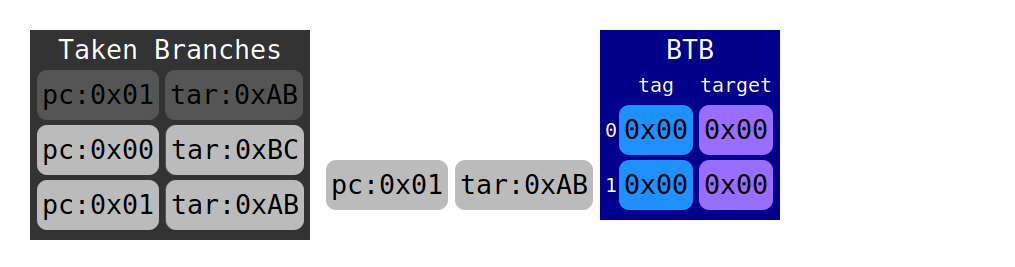
\includegraphics[width=0.7\textwidth]{chapter7_imgs/btb/btb000.png}
\caption{Branch Target Buffer is empty.}
\label{btb001}
\end{figure}

\begin{figure}[!ht]
\centering
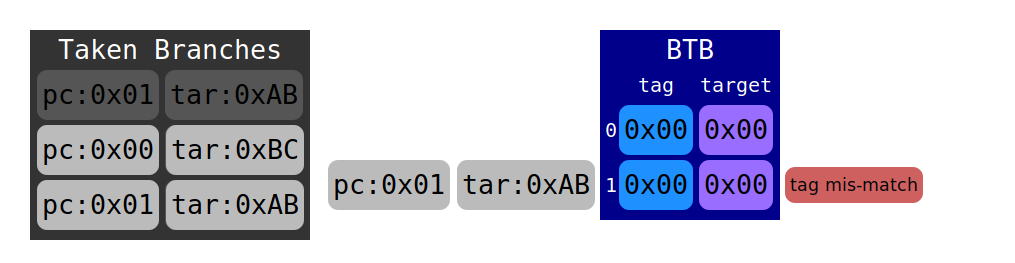
\includegraphics[width=0.7\textwidth]{chapter7_imgs/btb/btb001.png}
\caption{Tag-mismatch since the BTB was previously empty with tag bits $00$.}
\label{btb002}
\end{figure}

\begin{figure}[!ht]
\centering
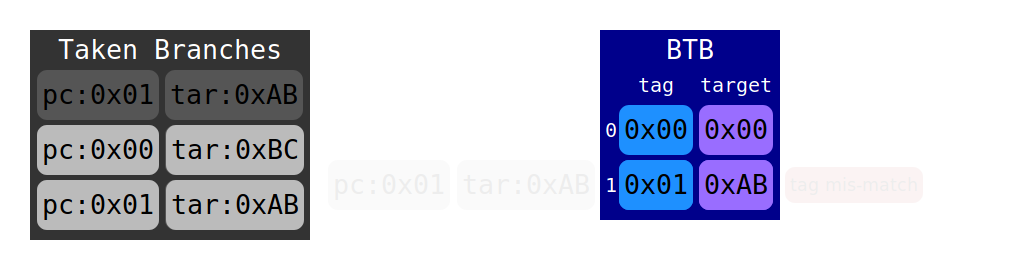
\includegraphics[width=0.7\textwidth]{chapter7_imgs/btb/btb002.png}
\caption{BTB is updated with previous \textit{tag} and \textit{target}.}
\label{btb003}
\end{figure}

\begin{figure}[!ht]
\centering
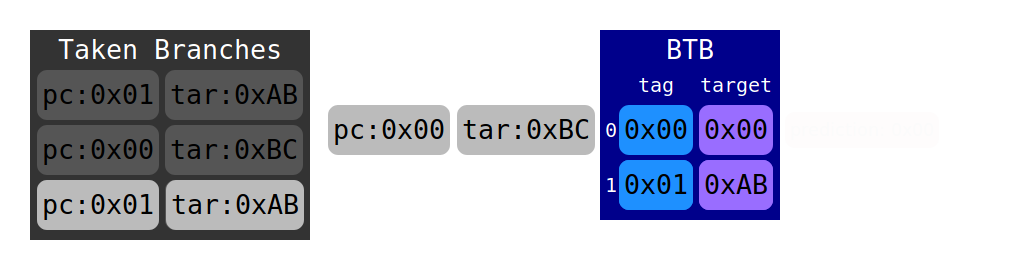
\includegraphics[width=0.7\textwidth]{chapter7_imgs/btb/btb003.png}
\caption{Next instruction arrives.}\
\label{btb004}
\end{figure}

\begin{figure}[!ht]
\centering
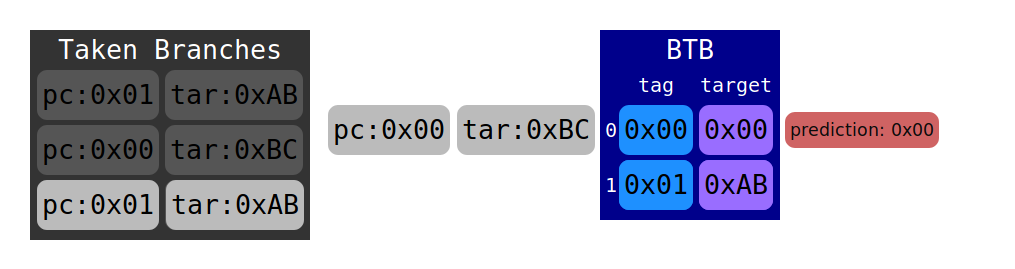
\includegraphics[width=0.7\textwidth]{chapter7_imgs/btb/btb004.png}
\caption{Mis-prediction because BTB is empty. Target is updated after this cycle.}
\label{btb005}
\end{figure}

\begin{figure}[!ht]
\centering
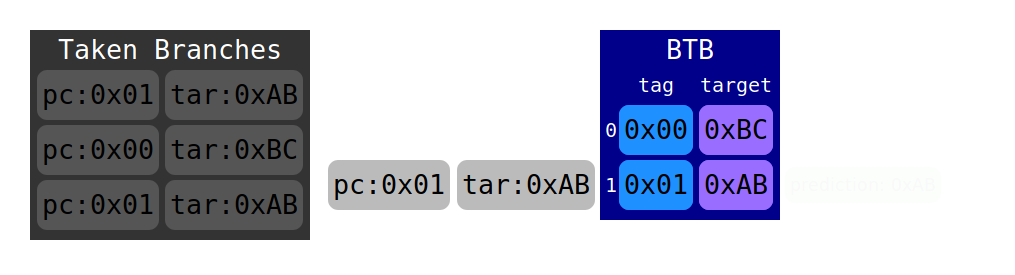
\includegraphics[width=0.7\textwidth]{chapter7_imgs/btb/btb005.png}
\caption{Next instruction arrives.}
\label{btb006}
\end{figure}

\begin{figure}[!ht]
\centering
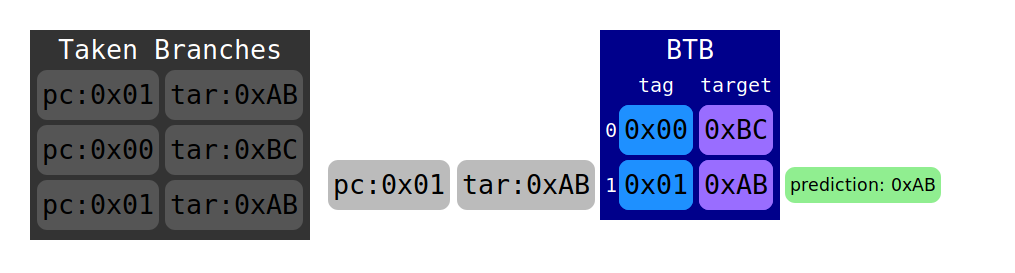
\includegraphics[width=0.7\textwidth]{chapter7_imgs/btb/btb006.png}
\caption{Correct branch prediction is made.}
\label{btb007}
\end{figure}

\end{answered}

\item What bits should you use as index bits and why do we discard the 2-bit least-significant bits?
\begin{answered}
The last 2 bits can be ignored because with MIPS, they are 32-bit instructions (PC is 32 bits) that are 4-bytes in size. You can throw away 2 bits because they will be the same (00) for all instructions since the instructions will all be incremented 4 bytes at a time. If you used these bits as BTB index bits, you would reduce your BTB target capacity implicitly. 

We select lower order 7-bits instead of higher order 7-bits because the lower order bits change a lot more than the higher order bits during a program. This can also be thought of as picking bits that have the highest \textit{entropy} and therefore can store the largest amount of information.

\textit{Is this the best way to do this hashing?} No, there are definitely better and more complicated ways to design a hashing function that better utilizes it's has indices. But this is a good start. 
\end{answered}

\item What is the purpose of the TAG entry in the Branch Target Buffer (BTB)?
\begin{answered}
%This will help us answer \textbf{(a) Is this a branch instruction?}
To understand the purpose of the \textbf{tag} entries, imagine a scenario where we did not have the \textit{tag} entries. While running a program with many instructions, a situation will arise where the \textit{Branch Target Buffer (BTB)} has been completely filled with entries (it is \textbf{saturated}). What this means for the following instructions is that every incoming instruction is treated as a taken branch and is mapped to a \textit{target}, however this is definitely not the case.

To avoid this situation, an additional \textbf{tag field} is introduced which associates a given \textit{Branch Target Buffer (BTB)} entry with a particular \textit{Program Counter (PC)}, which is used to tag that particular branching instruction. 

During the actual \textbf{\textit{BTB} update}, this will look like:
\begin{equation*}
\begin{split}
    BTB[PC].tag = & \ PC \\
    BTB[PC].target = & \ \text{target of branch} 
\end{split}
\end{equation*}

And at the \textbf{\textit{BTB} prediction step} in the \textit{Fetch Stage}, this will look like:
\begin{equation*}
    \begin{split}
        Predicted\ PC\ = (BTB[PC].tag == PC)\ ?\ BTB[PC].target\ :\ PC + 4
    \end{split}
\end{equation*}
\end{answered}
\vspace{-0.8cm}

\item Direct Targets and Indirect Targets
\begin{answered}
\textit{(a) Why does this simple \textit{Branch Target Buffer (BTB)} work?}

Most control instructions use \textbf{direct targets}, i.e they branch to the same targets each time (\textit{example:} JMP instructions). And the \textit{BTB} does this really well.

\qquad \textit{(b) What if this isn't the case?}

There are plenty of cases where control instructions use \textbf{indirect targets}:
\begin{itemize}
    \item When you are branching to a value in a \textit{Register}. There is no way to know this in the \textit{Fetch Stage}.
    \item Dynamically Linked Functions (DLLs) - here the control flow will usually jump to a table in memory to find out where to go next.
    \item Virtual Functions (C++) - the control flow will usually branch to a location depending on the data type provided to the function (for \textit{example}).
    \item Switch statements - difficult to handle but relatively uncommon
    \item Function returns - challenging because of the need to return to the caller; this varies heavily. This is difficult but we can use additional hardware called a \textbf{Return Address Stack (RAS)} to handle this.
\end{itemize}
\end{answered}

\item Return Address Stack (RAS)
\begin{answered}
The mechanism is a fairly straightforward stack operation. During a function call the next PC, \textit{(PC+4)}, is placed on top of the stack. A return instruction's target prediction is done by popping an element from the stack.

\textit{(a) How large is this stack?}

It has a fixed capacity and hence will not work well for large amounts of instructions. But we can throw away the oldest instructions to ensure a relatively good accuracy for recent instructions. At the end of the day these are \textit{predictions} anyway, so if it is \textit{incorrect} for old instructions, it is alright.

\textit{(b) How do we know when to use the RAS?}

There is usually another level of prediction that will associate a \textit{Program Counter (PC)} with whether the \textbf{Return Address Stack (RAS)} is to be used or not. This will involve additional bits and hardware. 
\end{answered}

\item Branch Direction Prediction
\begin{answered}
We use a similar strategy from \textit{branch target prediction} where we want to \textit{learn from the past and predict the future}. Instead of learning a mapping from \textit{Program Counter (PC)} to \textit{Target}, here we learn a mapping from \textit{Program Counter (PC)} to a single \textit{Taken or Not Taken} bit. 

Individual conditional branches are often very \textbf{biased}. Usually 90\% branch one way or the other.
\end{answered}

\item Bimodal Branch Predictor
\begin{answered}
This is the simplest form of \textit{branch direction prediction}, which is similar in design to the \textit{Branch Target Buffer (BTB)} except the \textbf{Branch History Table (BHT)} entry is a single bit for \textbf{Taken} or \textbf{Not Taken}. The following screenshots were taken from the \textit{http://comparchviz.com} tool.

The following \textit{example} assumes a \textbf{Branch History Table (BHT)} with \textbf{2} index bits. The \textbf{BHT} is initialized with all \textbf{Not Taken (N)}. The \textbf{3} \textit{Program Counters (PCs)} in the system are $12$, $23$ and $12$.

\begin{figure}[!ht]
\centering
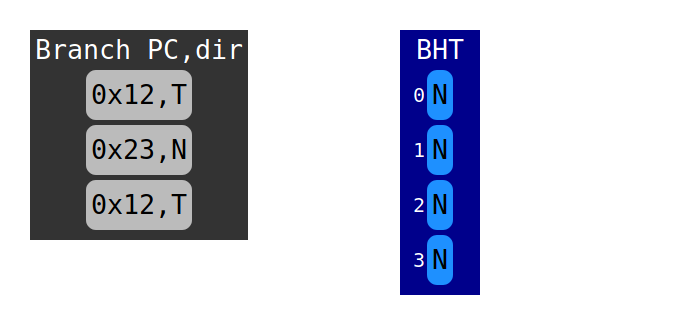
\includegraphics[width=0.45\textwidth]{chapter7_imgs/bbp/bbp000.png}
\caption{The Branch History Table (BHT) is initially set to all \textit{Not Taken}}
\label{bbp000}
\end{figure}

\begin{figure}[!ht]
\centering
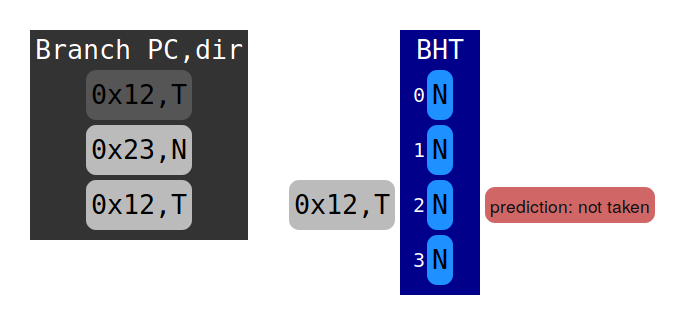
\includegraphics[width=0.45\textwidth]{chapter7_imgs/bbp/bbp001.png}
\caption{An instruction arrives but a false prediction is made}
\label{bbp001}
\end{figure}

\begin{figure}[!ht]
\centering
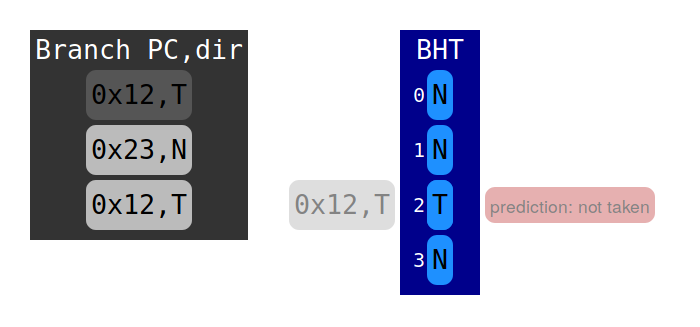
\includegraphics[width=0.45\textwidth]{chapter7_imgs/bbp/bbp002.png}
\caption{The table is then updated}
\label{bbp002}
\end{figure}

\begin{figure}[!ht]
\centering
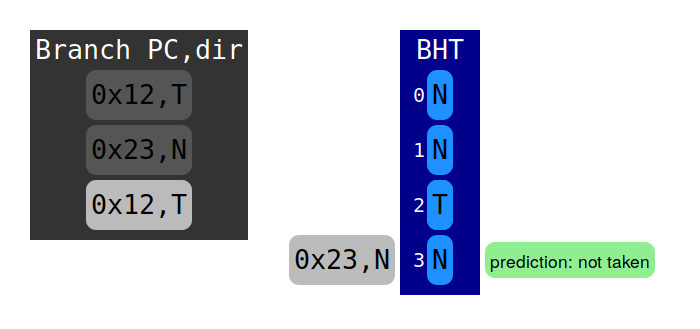
\includegraphics[width=0.45\textwidth]{chapter7_imgs/bbp/bbp003.png}
\caption{Another instruction arrives and a correct prediction is made}
\label{bbp003}
\end{figure}

\begin{figure}[!ht]
\centering
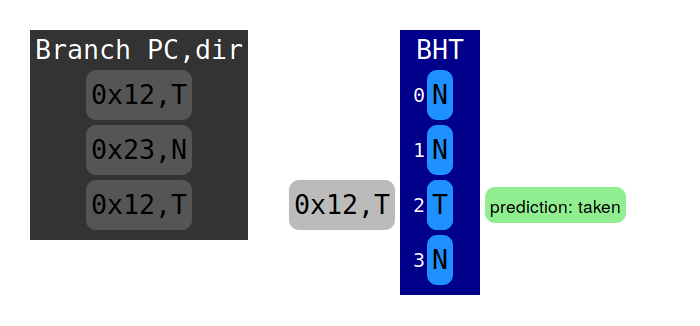
\includegraphics[width=0.45\textwidth]{chapter7_imgs/bbp/bbp004.png}
\caption{The first instruction arrives again and a correction prediction is made}
\label{bbp004}
\end{figure}
\end{answered}

\item Two-Bit Saturating Counter (2BC)
\begin{answered}

\textit{Failure of Bimodal Branch Predictor:}

An obvious situation in which the bimodal branch predictor will fail is in nested loops such as the following:
\begin{equation*}
\begin{split}
    & \text{for (i=0;i$<$100;i++)} \\
    & \quad \text{for (j=0;j$<$3;j++)} \\
    & \quad \quad ...
\end{split}
\end{equation*}

In the above situation, a bi-modal branch predictor will continuously switch between states and result in a low prediction accuracy.

The previous \textit{Branch History Table (BHT)} based approach can be thought of as \textbf{changing it's mind too quickly}. We can introduce a level of \textbf{resistance} and force the predictor to \textit{mis-predict twice before changing it's mind}. This is done by using a \textbf{2-bit saturating counter} that will essentially model a four-state finite state machine. The additional bits provide a larger memory.

\begin{equation*}
    (0,1,2,3) = (N,n,t,T)
\end{equation*}

The state-transition $(state,prediction)\rightarrow(state)$ function can be thought of as follows:
\begin{equation*}
    \begin{split}
        (N, NT) & \rightarrow N , \quad (T, NT) \rightarrow t \\
        (N, T) & \rightarrow n , \quad (T, T) \rightarrow T \\
        (n, NT) & \rightarrow N , \quad (t, NT) \rightarrow n \\
        (n, T) & \rightarrow t , \quad (t, T) \rightarrow T \\
    \end{split}
\end{equation*}
\end{answered}

\item GShare History-Based Predictor
\begin{answered}
While the last two methods of \textit{Bimodal Branch Predictor 1-bit} and \textit{2-bit Saturating Counters} did a reasonable job at learning previous history, there are conditions such as below where learning history is insufficient. We need to instead learn to identify recurring patterns of instructions.

In the \textit{example} below, the modulo three conditional branch is repeated twice as seen in \textit{(i) and (ii)}, but they are separated by some unrelated, unpredictable set of instructions. In this case, the above two methods would not be able to effectively predict the right branch targets even though it has previously seen the same instructions.

\begin{equation*}
\begin{split}
    & \text{for(i=0;i$<$10000;i++)} \\
    & \{ \\
    & \quad\textbf{if(i\%3==0)}\ \{ \quad\quad \textit{--- (i)}\\
    & \quad\textit{...} \\
    & \quad \} \\
    & \quad ... \\
    & \quad \textit{... unrelated sequence ...} \\
    & \quad ... \\
    & \quad\textbf{if(i\%3==0)}\ \{ \quad\quad \textit{--- (ii)}\\
    & \quad\textit{...} \\
    & \quad \} \\ 
    & \}
\end{split}
\end{equation*}

GShare maintains a \textbf{Branch History Register (BHR)} in addition to a \textbf{Branch History Table (BHT)}, which typically will use \textbf{2-bit Saturating Counters}.

\textit{How do we incorporate this idea of history and correlation into our predictions?}

Instead of using just the \textit{Program Counter (PC)} as the index into the \textit{Branch History Table (BHT)}, use PC $\oplus$ BHR (xor operation) as the index to the BHT. This will result in more unique \textit{keys / indexes} into the table.

We need to train the counter (BHT) and the BHR (\textit{Branch History Register}) after each branch instruction.
\end{answered}

\item GShare Example
\begin{answered}
This example is taken from \textit{http://comparchviz.com}.
\end{answered}

\item Hybrid Tournament Predictor
\begin{answered}
A simple \textit{bimodal branch predictor} is good for short term history dependent branches and is fast. Most static target branch prediction can be accomplished by this method. A \textit{gshare correlated branch predictor} is good for branch prediction that requires pattern identification and correlated branches over time. \textit{Can we combine the two?}

A \textbf{Hybrid Predictor} combines the above mentioned predictors and introduces a third component called the \textbf{chooser} which learns to predict which of the above two methods to use. This allows the correlated predictor to become smaller than previously defined and results in 90-95\% accuracy. 
\end{answered}

\item Reducing Branch Penalty
\begin{answered}
Even a taken branch results in a \textbf{2 cycle} branch penalty. Can we decide a faster branching strategy that can decide at the \textit{Decode Stage} and not the \textit{Execute Stage} on instructions that require some test conditions?

What if we evaluate test conditions that are checking for \textit{equality} or a \textit{comparison} and we do this in the \textit{Decode Stage}? This would reduce the branch penalty to \textbf{1 cycle} in these cases.

\textit{Performance:}

Let's say that Branches: 20\% and 75\% of branches are taken. Out of these branches, 25\% cannot be optimized with the method above and require an additional cycle.

\begin{equation*}
    CPI = 1 + \text{fast branch instructions} + \text{regular instructions}
\end{equation*}
\begin{equation*}
    CPI = 1 + (0.20 \times 0.75 \times 1) + (0.20 \times 0.25 \times 1) = 1.2
\end{equation*}

\textit{Branch Predictions} are still a big problem even with all these optimizations. For typically large pipelines, mis-predictions cost the system 10+ cycles!
\end{answered}

\item Predication
\begin{answered}
\textit{Instead of predicting which way we're going, why not go both ways?}

Predication is an \textbf{alternate view} that attempts to get rid of branch prediction by rephrasing control flow instructions as conditional instructions. The condition is represented by a \textbf{predicate bit} and these instructions will either execute as normal or as \textit{no-ops} depending on this predicate bit.

For control sequences such as an \textbf{if-then} statement, there will be no overhead and therefore there are gains in performance to be had. 

However, in \textbf{if-then-else} statements, since there is only \textbf{one} useful path, this might not be very effective. 

Predicated instructions are useful only if the number of cycles saved is more than the mis-prediction penalty if we were using regular branch predictors. 

\end{answered}

\end{QandA}

\newpage 

\section{Textbook Notes}
\begin{QandA}
\item Control Hazards
\begin{answered}
Control hazards occur less frequently than data hazards, and there is nothing as effective against control hazards as forwarding / bypassing is against data hazards.
\end{answered}

\item Fast Branching
\begin{answered}
Many branch instructions rely on simple tests (\textit{equality or sign, for example}) and such tests do not require a full \textbf{ALU} and can be done independently with a few gates. For these instructions, we can reduce the cost by one cycle. 

When a more complex branch decision is required, a separate instruction that uses an ALU to perform a comparison is used.
\end{answered}

\item Drawback of 1-bit Bimodal Branch Predictor
\begin{answered}
Even if a branch is almost always taken, we can predict incorrectly twice, rather than once, when it is not taken. 

\textit{Consider a loop branch that branches nine times in a row, then is not taken once. What is the prediction accuracy for this branch, assuming the prediction bit for this branch remains in the prediction buffer?}

There will be a mis-prediction at the entry to this loop and one at the end, resulting in 80\% accuracy even though the branch is taken 90\% of the time. We should be able to do better than this? \textbf{Yes, use 2-bit saturating counter.}
\end{answered}

\item 2-bit Saturating Counter Branch Predictor
\begin{answered}
\begin{figure}[!ht]
\centering
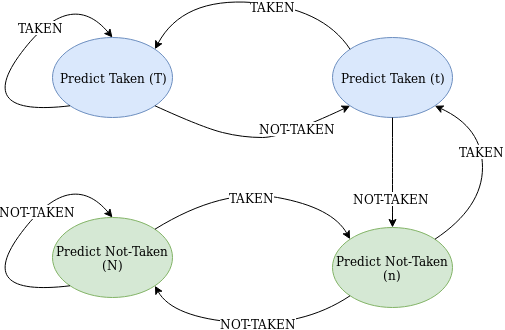
\includegraphics[width=0.4\textwidth]{chapter7_imgs/2bitsatcounter.png}
\caption{Finite State Machine for 2-bit Saturating Counter}
\label{2bitsatcounter}
\end{figure}
\end{answered}

\end{QandA}

\newpage 

\section{Exam Questions}
\begin{QandA}
\item List one source of slowdown that increases as pipeline depth increases
\begin{answered}
Branch mis-prediction penalty
\end{answered}

\item A bimodal branch predictor augmented with a branch history register is known as what kind of predictor?
\begin{answered}
GShare Branch Predictor
\end{answered}

\item What does BTB stand for?
\begin{answered}
Branch Target Buffer
\end{answered}

\item What are the three steps / questions involved with Branch Prediction?
\vspace{-0.85cm}
\begin{answered}
\begin{enumerate}
    \item Is this instruction a branch?
    \item If it is a branch, is it taken or not taken?
    \item If it is taken, where is it going?
\end{enumerate}
\end{answered}

\item Your pipelined processor in Lab 4 implements speculative branch prediction (true / false)?
\begin{answered}
True, because even just predicting $PC=PC+1$ is a form of speculation.  
\end{answered}

\end{QandA}

\end{document}
